\begin{frame}[fragile] 
\secframetitle{\ssCharm}
\framesubtitle{\charm\ collections of chares}
\vspace{-0.2in}
\begin{center}
\begin{minipage}{4in}
\begin{minipage}{1.5in}
\bluebf{Chare Arrays}
\end{minipage} \ 
\begin{minipage}{2in}

\includegraphics[width=2.0in]{chare-array.pdf}
\end{minipage}
\vspace{0.1in}
  \begin{itemize}
  \item \bluetext{distributed array of chares}
  \item \bluetext{migratable elements}
  \item \bluetext{flexible indexing}
  \end{itemize}
\vspace{0.2in}
\begin{minipage}{1.5in}
\redbf{Chare Groups}
\end{minipage} \ 
\begin{minipage}{2in}
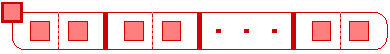
\includegraphics[width=2.0in]{chare-group.pdf}
\end{minipage}
  \begin{itemize}
\setbeamercolor*{item}{fg=red!50!black}
  \item \redtext{one chare per processor (non-migratable)}
  \end{itemize}
\vspace{0.2in}
\begin{minipage}{1.5in}
\greenbf{Chare Nodegroups}
\end{minipage} \ 
\begin{minipage}{2in}
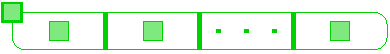
\includegraphics[width=2.0in]{chare-nodegroup.pdf}
\end{minipage}
  \begin{itemize}
\setbeamercolor*{item}{fg=green!50!black}
  \item \greentext{one chare per node (non-migratable)}
  \end{itemize}
\end{minipage}
\end{center}

\end{frame}
